% Template for PLoS
% Version 3.4 January 2017
% -- FIGURES AND TABLES
%
% Please include tables/figure captions directly after the paragraph where they are first cited in the text.
%
% DO NOT INCLUDE GRAPHICS IN YOUR MANUSCRIPT
% - Figures should be uploaded separately from your manuscript file. 
% - Figures generated using LaTeX should be extracted and removed from the PDF before submission. 
% - Figures containing multiple panels/subfigures must be combined into one image file before submission.
% For figure citations, please use "Fig" instead of "Figure".
% See http://journals.plos.org/plosone/s/figures for PLOS figure guidelines.
%
% Tables should be cell-based and may not contain:
% - spacing/line breaks within cells to alter layout or alignment
% - do not nest tabular environments (no tabular environments within tabular environments)
% - no graphics or colored text (cell background color/shading OK)
% See http://journals.plos.org/plosone/s/tables for table guidelines.
%
% For tables that exceed the width of the text column, use the adjustwidth environment as illustrated in the example table in text below.
%
% % % % % % % % % % % % % % % % % % % % % % % %

\documentclass[10pt,letterpaper]{article}\usepackage[]{graphicx}\usepackage[]{color}
%% maxwidth is the original width if it is less than linewidth
%% otherwise use linewidth (to make sure the graphics do not exceed the margin)
\makeatletter
\def\maxwidth{ %
  \ifdim\Gin@nat@width>\linewidth
    \linewidth
  \else
    \Gin@nat@width
  \fi
}
\makeatother

\definecolor{fgcolor}{rgb}{0.345, 0.345, 0.345}
\newcommand{\hlnum}[1]{\textcolor[rgb]{0.686,0.059,0.569}{#1}}%
\newcommand{\hlstr}[1]{\textcolor[rgb]{0.192,0.494,0.8}{#1}}%
\newcommand{\hlcom}[1]{\textcolor[rgb]{0.678,0.584,0.686}{\textit{#1}}}%
\newcommand{\hlopt}[1]{\textcolor[rgb]{0,0,0}{#1}}%
\newcommand{\hlstd}[1]{\textcolor[rgb]{0.345,0.345,0.345}{#1}}%
\newcommand{\hlkwa}[1]{\textcolor[rgb]{0.161,0.373,0.58}{\textbf{#1}}}%
\newcommand{\hlkwb}[1]{\textcolor[rgb]{0.69,0.353,0.396}{#1}}%
\newcommand{\hlkwc}[1]{\textcolor[rgb]{0.333,0.667,0.333}{#1}}%
\newcommand{\hlkwd}[1]{\textcolor[rgb]{0.737,0.353,0.396}{\textbf{#1}}}%
\let\hlipl\hlkwb

\usepackage{framed}
\makeatletter
\newenvironment{kframe}{%
 \def\at@end@of@kframe{}%
 \ifinner\ifhmode%
  \def\at@end@of@kframe{\end{minipage}}%
  \begin{minipage}{\columnwidth}%
 \fi\fi%
 \def\FrameCommand##1{\hskip\@totalleftmargin \hskip-\fboxsep
 \colorbox{shadecolor}{##1}\hskip-\fboxsep
     % There is no \\@totalrightmargin, so:
     \hskip-\linewidth \hskip-\@totalleftmargin \hskip\columnwidth}%
 \MakeFramed {\advance\hsize-\width
   \@totalleftmargin\z@ \linewidth\hsize
   \@setminipage}}%
 {\par\unskip\endMakeFramed%
 \at@end@of@kframe}
\makeatother

\definecolor{shadecolor}{rgb}{.97, .97, .97}
\definecolor{messagecolor}{rgb}{0, 0, 0}
\definecolor{warningcolor}{rgb}{1, 0, 1}
\definecolor{errorcolor}{rgb}{1, 0, 0}
\newenvironment{knitrout}{}{} % an empty environment to be redefined in TeX

\usepackage{alltt}
\usepackage[top=0.85in,left=2.75in,footskip=0.75in]{geometry}

\usepackage{amsmath,amssymb}
\usepackage{changepage}
\usepackage[utf8x]{inputenc}
\usepackage{textcomp,marvosym}
\usepackage{cite}
\usepackage{nameref,hyperref}
\usepackage[right]{lineno}
\usepackage{microtype}
\DisableLigatures[f]{encoding = *, family = * }
\usepackage[table]{xcolor}
\usepackage{array}

% create "+" rule type for thick vertical lines
\newcolumntype{+}{!{\vrule width 2pt}}

% create \thickcline for thick horizontal lines of variable length
\newlength\savedwidth
\newcommand\thickcline[1]{%
  \noalign{\global\savedwidth\arrayrulewidth\global\arrayrulewidth 2pt}%
  \cline{#1}%
  \noalign{\vskip\arrayrulewidth}%
  \noalign{\global\arrayrulewidth\savedwidth}%
}

% \thickhline command for thick horizontal lines that span the table
\newcommand\thickhline{\noalign{\global\savedwidth\arrayrulewidth\global\arrayrulewidth 2pt}%
\hline
\noalign{\global\arrayrulewidth\savedwidth}}

% Remove comment for double spacing
%\usepackage{setspace} 
%\doublespacing

% Text layout
\raggedright
\setlength{\parindent}{0.5cm}
\textwidth 5.25in 
\textheight 8.75in

% Bold the 'Figure #' in the caption and separate it from the title/caption with a period
% Captions will be left justified
\usepackage[aboveskip=1pt,labelfont=bf,labelsep=period,justification=raggedright,singlelinecheck=off]{caption}
\renewcommand{\figurename}{Fig}

% Use the PLoS provided BiBTeX style
\bibliographystyle{plos2015}

% Remove brackets from numbering in List of References
\makeatletter
\renewcommand{\@biblabel}[1]{\quad#1.}
\makeatother

% Leave date blank
\date{}

% Header and Footer with logo
\usepackage{lastpage,fancyhdr,graphicx}
\usepackage{epstopdf}
\pagestyle{myheadings}
\pagestyle{fancy}
\fancyhf{}
\setlength{\headheight}{27.023pt}
\lhead{
\includegraphics[width=2.0in]{PLOS-submission.eps}}
\rfoot{\thepage/\pageref{LastPage}}
\renewcommand{\footrule}{\hrule height 2pt \vspace{2mm}}
\fancyheadoffset[L]{2.25in}
\fancyfootoffset[L]{2.25in}
\lfoot{\sf PLOS}


\usepackage[colorinlistoftodos]{todonotes}
%\usepackage[colorinlistoftodos,disable]{todonotes}

%% Include all macros below
\newcommand{\citationneeded}[2][]{\todo[color=brown, fancyline, #1]{\textbf{Citation Needed:} #2}}


\newcommand{\lorem}{{\bf LOREM}}
\newcommand{\ipsum}{{\bf IPSUM}}

%% END MACROS SECTION
\IfFileExists{upquote.sty}{\usepackage{upquote}}{}
\begin{document}
\vspace*{0.2in}

% Title must be 250 characters or less.
\begin{flushleft}
{\Large
\textbf\newline{Rethomics: an R framework to analyse high-throughput behavioural data} 
}
\newline
% Insert author names, affiliations and corresponding author email (do not include titles, positions, or degrees).
\\
Quentin Geissmann\textsuperscript{1*},
Luis Garcia Rodriguez\textsuperscript{2},
Esteban J Beckwith\textsuperscript{1},
Giorgio F Gilestro\textsuperscript{1*}
\\
\bigskip
\textbf{1} Department of Life Sciences, Imperial College London, London, United Kingdom
\\
\textbf{2} Affiliation Dept/Program/Center, Institution Name, City, State, Country %TODO @luis
\\
\bigskip


% Use the asterisk to denote corresponding authorship and provide email address in note below.
* qgeissmann@gmail.com, giorgio@gilest.ro

\end{flushleft}
% Please keep the abstract below 300 words
\section*{Abstract}
Ethomics, a quantitative and high-throughput approach to animal behaviour, is a new and exciting field.
The recent development of automatised methods that can score various behaviours on a large number of animals
% brings the promise of a powerful and original insight
provides biologists with an unprecedented set of tools to decipher these complex phenotypes. 
Analysing ethomics data comes with many challenges that are largely shared across acquisition platform and paradigms.
However, there is little effort in providing a generic framework to specifically analyse multiple and long behavioural time series.
We developed the \texttt{rethomics} framework, a suite of \texttt{R} packages that altogether offer utilities to:
import, store, visualise and analyse behavioural data.
In this article, we describe it and show an example of its application to the blooming field of sleep and circadian rhythm in fruit fly.
The \texttt{rethomics} framework is available and documented at \href{https://rethomics.github.io}{https://rethomics.github.io}.



% Please keep the Author Summary between 150 and 200 words
% Use first person. PLOS ONE authors please skip this step. 
% Author Summary not valid for PLOS ONE submissions.   
%\section*{Author summary}
%Lorem ipsum dolor sit amet, consectetur adipiscing elit. Curabitur eget porta erat. Morbi consectetur est vel gravida pretium. Suspendisse ut dui eu ante cursus gravida non %sed sem. Nullam sapien tellus, commodo id velit id, eleifend volutpat quam. Phasellus mauris velit, dapibus finibus elementum vel, pulvinar non tellus. Nunc pellentesque %pretium diam, quis maximus dolor faucibus id. Nunc convallis sodales ante, ut ullamcorper est egestas vitae. Nam sit amet enim ultrices, ultrices elit pulvinar, volutpat risus.

\linenumbers

% Use "Eq" instead of "Equation" for equation citations.
\section*{Introduction}

Animal behaviours are complex phenotypical manifestations of the interaction between nervous systems and their external or internal environment.
In the last few decades, our ability to record vast quantities of various phenotypical data has tremendously increased.
Behaviour scoring is certainly not an exception to this trend.
Indeed, many platforms (TODO citations) have been developed in order to allow biologists to continuously record behaviours such as activity, position and feeding of multiple animals over long durations (days or weeks).

The availability of large amounts of data is very exciting as it paves the way for in-depth analyses.
Clearly, the multiplicity of model organisms, hypotheses and paradigms should be matched by a diverse range of recording tools.
However, when it comes to the subsequent data analysis, there is no unified, programmatic, framework that could be used as a set of building blocks in a pipeline.
Instead, tools tend to consist of graphical interfaces with rigid functionalities that only import data from a single platform.
There are, at least, three issues with this approach.
First of all, state-of-the-art analysis and visualisation requires a level of reproducibility, flexibility and scalability than only a programmatic interface can provide.
Secondly, it favours replicated work as developers need to create their independent solution to similar problems.
Lastly, it links analysis and visualisation to the target acquisition tool, which makes it very difficult to share cross-tool utilities and concepts.

Thankfully, behavioural data is conceptually largely agnostic of the acquisition platform and paradigm. 	
Typically, the behaviour of each individual is described by a long time series (possibly multivariate and heterogeneous).
Importantly, individuals are labelled with arbitrary metadata defined by the experimenter (\emph{e.g.} sex, treatment and genotype).
Efficiently combining and manipulating these two types of information, on datasets of hundreds of individuals, each recorded for weeks, is not trivial.

In the article herein, we describe \texttt{rethomics}, a framework that unifies analysis of behavioural dataset in an efficient and flexible manner.
It offers an elegant computational solution to store, manipulate and visualise a large amount of data.
We expect it to fill the gap between behavioural biology and data sciences, thus promoting collaboration between computational and behavioural biologists.
\texttt{rethomics} comes with a extensive documentation and a set of both practical and theoretical tutorials.


\section*{Design and Implementation}

\texttt{rethomics} is implemented as a collection of small packages linked to one another (Fig~\ref{fig:fig-1}).
This paradigm follows the model of modern frameworks such as the \texttt{tidyverse}, which results in increased testability and maintainability.
In it, the different tasks of the analysis workflow (\emph{i.e.} data import, manipulation and visualisation)
are explicitly handled by different packages.
At the core of \texttt{rethomics}, the \texttt{behavr} package offers a very flexible and efficient solution to store large amounts data (\emph{e.g.} position and activity) as well as metadata (\emph{e.g.} treatment, genotype and so on) in a single \texttt{data.table}-derived object.
Any input package will import experimental data as a \texttt{behavr} table which can, in turn, be manipulated and visualised regardless of the original input platform.
Results and plots integrate seamlessly within the \texttt{R} ecosystem, hence providing users with state-of-the-art visualisation and statistics tools.

% Place figure captions after the first paragraph in which they are cited.


     
\begin{figure}[!h]
    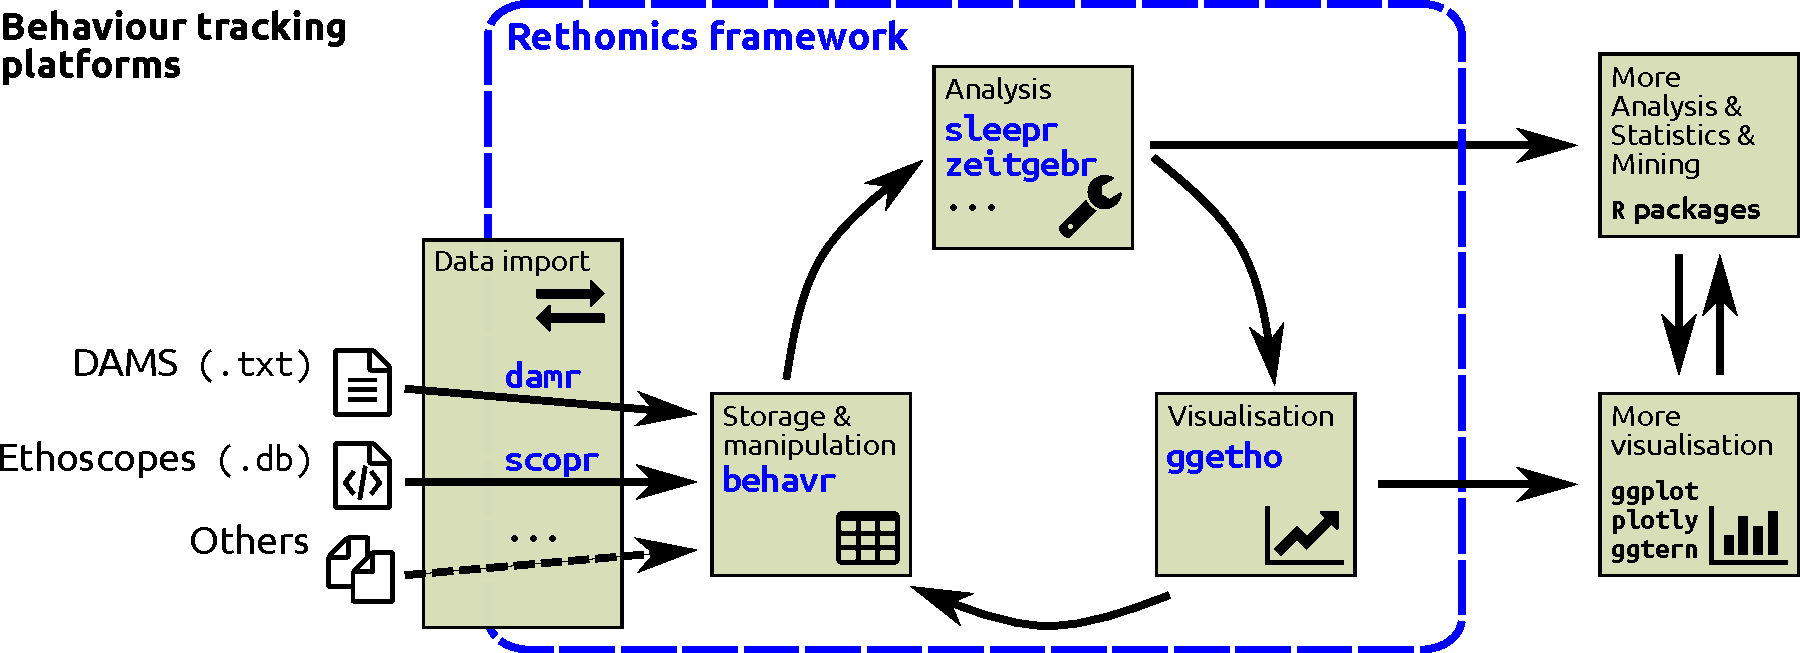
\includegraphics[width=1\textwidth]{fig/fig-1.pdf}
	\caption{{\bf The \texttt{rethomics} workflow.}
		Diagram representing, from left to right, the interplay between the raw data, the \texttt{rethomics} packages (in blue) and the rest of the \texttt{R} ecosystem.}
	\label{fig:fig-1}
\end{figure}


\subsection*{Internal data structure}
We created \texttt{behavr} (Fig~\ref{fig:fig-2}), a new data structure, based on the widely adopted \texttt{data.table} object, in order to address 
two challenges that are inherent to manipulating ethomics results.

Firstly, there could be very long (typically $k_i > 10^8, \forall i \in [1,n]$), multivariate (often, $q > 10$), time series for each individual.
For instance, each series could represent variables that encode coordinates, orientation, dimensions, activity, colour intensity and so on, sampled several times per second, over multiple days. Therefore, data structure must be computationally efficient -- both in term of memory footprint and processing speed. 

Secondly, a large amount of individuals are often studied (typically $n > 100$).
Each individual ($i$) is associated with metadata, that is a set of $p$ ``metavariables'' that describe experimental conditions.
For instance, metadata stores information regarding the date and location of the experiment, treatment, genotype, sex, \emph{post hoc} observations and other arbitrary metavariables.
It is good practice to record as many metavariables as possible so they can later be used as covariates. 
Therefore, typically $p > 10$.
 
\texttt{behavr} tables link metadata and data within the same object, extending the syntax of \texttt{data.table} to manipulate, join and access metadata.
This approach guaranties that any data point can be mapped correctly to its parent metadata.
It also allows implicit update of metadata when data is altered.
For instance, when is data filtered, only the remaining individuals should be in the new metadata. 
It is also important that metadata and data can interoperate.
For instance, when one wants to update variable according to the value of a metavariable (say, alter the variable $x$ only for animals with the metavariable $sex=``male"$).

     
\begin{figure}[!h]
	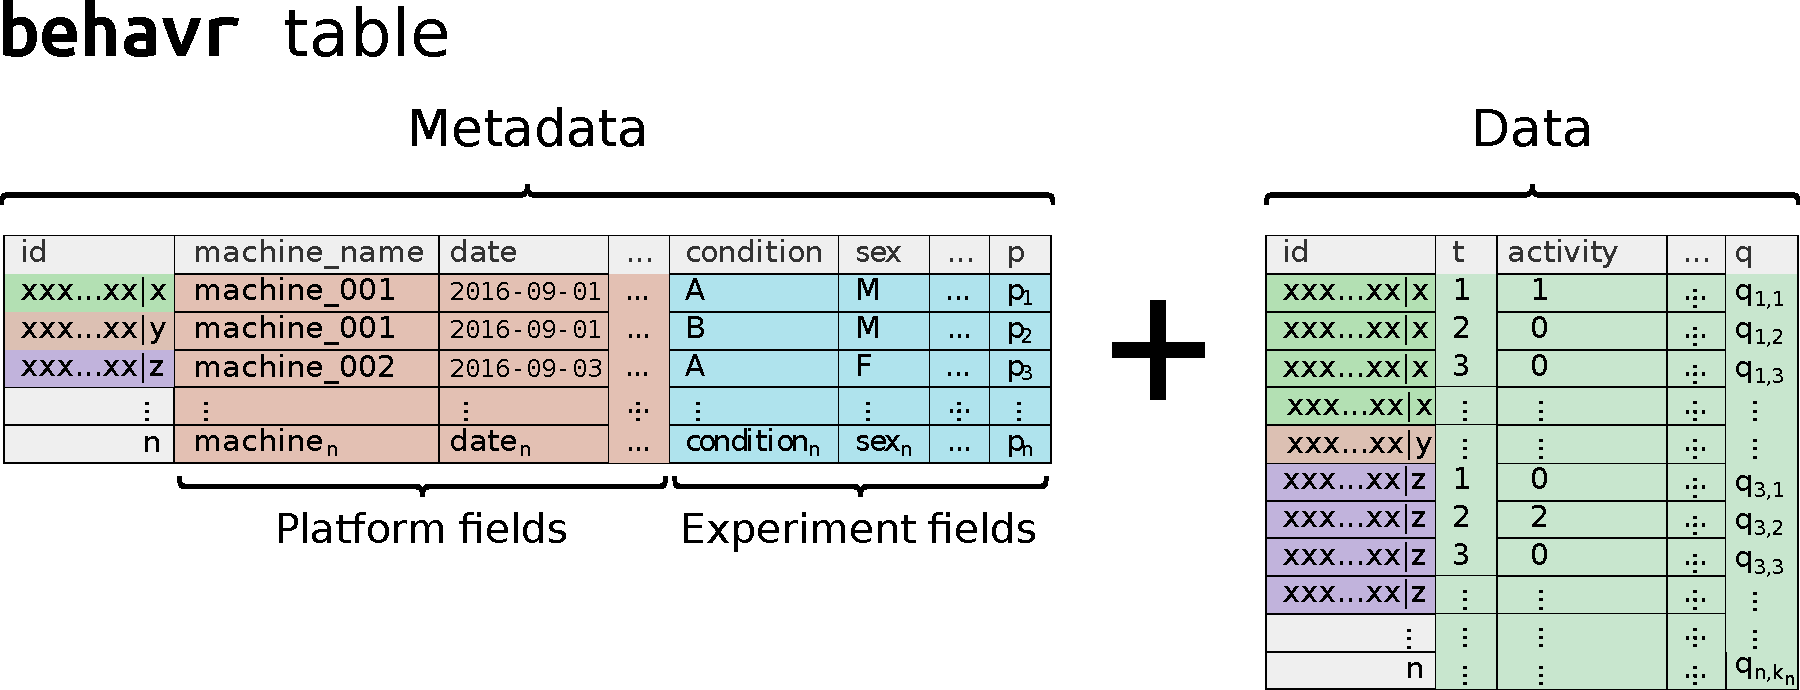
\includegraphics[width=1\textwidth]{fig/fig-2.pdf}
	\caption{{\bf Example of a \texttt{behavr} table.}
		The metadata holds a single row for each of the $n$ individuals. 
		Its columns, the $p$ metavariables, are of two kind: either required and defined by the acquisition platform (\emph{i.e.} used to fetch the data) or user-defined (\emph{i.e.} arbitrary).
		In the data, each row is a ``read'' (\emph{i.e.} information about one individual at one time point).
		It is formed of $q$ variables and is expected to have a very large number of reads $k$ for each individual.
		Data and metadata are implicitly joined with the \texttt{id} field.
		In this figure, the names used for variables and metavariable are only plausible examples that will likely differ in practice. 
	}
	\label{fig:fig-2}
\end{figure}


\subsection*{Data import}
Data import package translate results from a recording platform (\emph{e.g.} text files and databases) into a single \texttt{behavr} object.
Currently, we provide a package to read Drosophila Activity Monitor (DAM2) data  and another one for Ethoscope data.
Although the structure of the raw results if very different, conceptually, loading data is very similar.
In all cases the user is asked to generate a metadata table (one row per individual). 
In it, there will be both mandatory and optional columns.
The mandatory ones are the necessary and sufficient information to fetch data (\emph{e.g.} machine id, region of interest and date). 
The optional columns are user-defined arbitrary fields that relate to the experiment itself (\emph{e.g.} condition and sex).

In this respect, the metadata file is a standardised an comprehensive data frame describing an experiment.
Using such a structure comes with multiple advantages.
For instance, it simplify collaboration and data exchange as all treatments and individuals are very explicit.
Then, it promotes good experimental practices such as interspersion of treatments (indeed, without it, users are tempted to simplify their design by, for instance, confounding device/location and treatment).
Furthermore, it streamlines the inclusion and analysis of further replicates in the same workflow. Indeed, additional replicates can simply be added as new rows and replicate ID later used, if needed, as a covariate.	


\subsection*{Visualisation}
Long time series often need to be preprocessed before visualisation.
Typically, users are interested in understanding individual or population trends over time.
To integrate visualisation in \texttt{rethomics},
we implemented \texttt{ggetho}, a package extending the widely adopted \texttt{ggplot2} by providing preprocessing tools as well as new layers and scales.
Our tools make full use of the internal \texttt{behavr} structure to deliver efficient representations of temporal trends.
It particularly applies to the visualisation of long experiments, with the ability to, for instance, annotate light and dark phases, wrap time over a circadian day, display ``double-plotted actograms'' and periodograms. 
Importantly, \texttt{ggetho} is fully compatible with \texttt{ggplot2}.

\subsection*{Circadian and sleep analysis}
The packages \texttt{zeitgebr} and \texttt{sleepr} provide tools to analyse circadian behaviours and sleep, respectively.
Together, they offer a suite of methods to compute periodograms and find their peaks, score sleep from inactivity (\emph{e.g.} using the ``five minute rule''), and characterise the architecture of sleep bouts (\emph{e.g.} number, length and latency).






\section*{Results}

TODO description of the dataset here

* experiment goal

* design

* source

* express the idea that shis is just simple example that could be scaled up



First of all, we load the necessary libraries (see availability section for installation instructions):
\begin{knitrout}
\definecolor{shadecolor}{rgb}{0.969, 0.969, 0.969}\color{fgcolor}\begin{kframe}
\begin{alltt}
\hlkwd{library}\hlstd{(damr)}      \hlcom{# input DAM2 data}
\hlkwd{library}\hlstd{(zeitgebr)}  \hlcom{# periodogram computation}
\hlkwd{library}\hlstd{(sleepr)}    \hlcom{# sleep analysis}
\hlkwd{library}\hlstd{(ggetho)}    \hlcom{# behaviour visualisation}
\end{alltt}
\end{kframe}
\end{knitrout}

Then, the metadata file is read and linked to the \texttt{.txt} result files.

\begin{knitrout}
\definecolor{shadecolor}{rgb}{0.969, 0.969, 0.969}\color{fgcolor}\begin{kframe}
\begin{alltt}
\hlstd{metadata} \hlkwb{<-} \hlkwd{link_dam2_metadata}\hlstd{(}\hlstr{"metadata.csv"}\hlstd{,}\hlstr{"."}\hlstd{)}    \hlcom{# linking}
\hlcom{# print(metadata)                                     # check metadata}
\hlstd{dt} \hlkwb{<-} \hlkwd{load_dam2}\hlstd{(metadata)}                             \hlcom{# loading}
\hlkwd{summary}\hlstd{(dt)}                                           \hlcom{# quick summary}
\end{alltt}
\begin{verbatim}
## behavr table with:
##  58	individuals
##  8	metavariables
##  2	variables
##  1.58722e+05	measurements
##  1	key (id)
\end{verbatim}
\end{kframe}
\end{knitrout}

\subsection*{Preprocessing}
We notice, from the metadata, that the two replicates do not have the same time in baseline.
We would like to express the time relative to the important event: the transition to \texttt{LL}. 
To do so, we subtract the \texttt{baseline\_days} metavariable from the \texttt{t} variable.
This gives us an opportunity to illustrate the use \texttt{xmv()}, which expands metavariables as variables.
In addition, we use the \texttt{data.table} syntax to create, in place, a \texttt{moving} variable.
It is \texttt{TRUE} when and only when \texttt{activity} is greater than zero:

\begin{knitrout}
\definecolor{shadecolor}{rgb}{0.969, 0.969, 0.969}\color{fgcolor}\begin{kframe}
\begin{alltt}
\hlcom{# baseline subtraction -- note the use of xmv}
\hlstd{dt[,t} \hlkwb{:=} \hlstd{t} \hlopt{-} \hlkwd{days}\hlstd{(}\hlkwd{xmv}\hlstd{(baseline_days))]}
\hlstd{dt[, moving} \hlkwb{:=}  \hlstd{activity} \hlopt{>} \hlnum{0}\hlstd{]}
\end{alltt}
\end{kframe}
\end{knitrout}

\begin{knitrout}
\definecolor{shadecolor}{rgb}{0.969, 0.969, 0.969}\color{fgcolor}\begin{kframe}
\begin{alltt}
\hlkwd{summary}\hlstd{(dt)}
\end{alltt}
\begin{verbatim}
## behavr table with:
##  58	individuals
##  8	metavariables
##  3	variables
##  1.58722e+05	measurements
##  1	key (id)
\end{verbatim}
\end{kframe}
\end{knitrout}

To simplify visualisation, we create our own \texttt{label} metavariable, as combination of a number and \texttt{genotype}.
In the restricted context of this analysis, \texttt{label} acts a unique identifier.
Importantly, we keep \texttt{id} , which is more rigorous and universal.



\begin{knitrout}
\definecolor{shadecolor}{rgb}{0.969, 0.969, 0.969}\color{fgcolor}\begin{kframe}
\begin{alltt}
\hlstd{dt[, label} \hlkwb{:=} \hlkwd{interaction}\hlstd{(}\hlnum{1}\hlopt{:}\hlstd{.N, genotype),} \hlkwc{meta}\hlstd{=T]}
\hlkwd{print}\hlstd{(dt)}
\end{alltt}
\end{kframe}
\end{knitrout}


\subsection*{Curation}
It is important to visualise an overview of how each individual behaved and, if necessary, alter the data accordingly. For this, we generate a tile plot (Fig~\ref{fig:fig-3}A).

\begin{figure}[!h]
	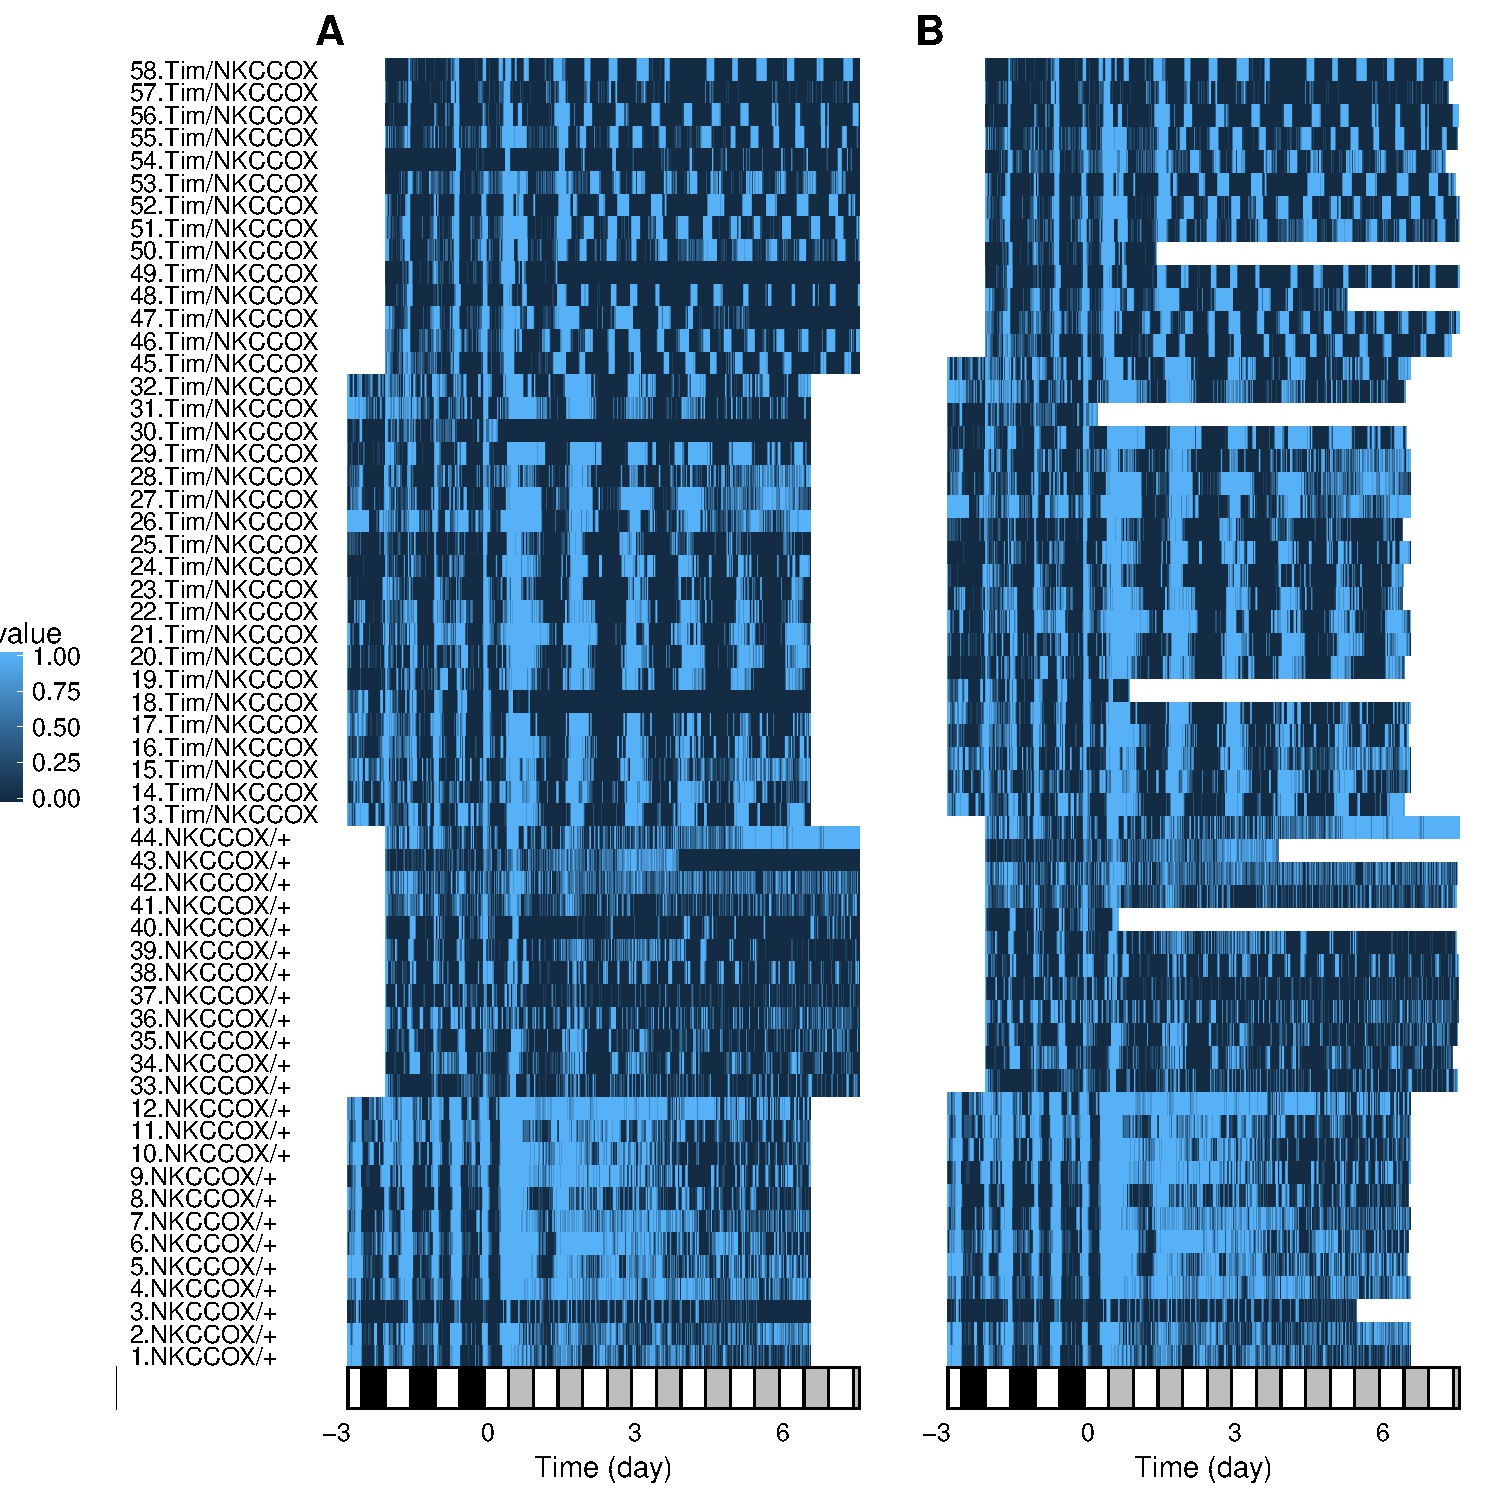
\includegraphics[width=1\textwidth]{fig/fig-3.pdf}
	\caption{{\bf Experiment quality control.}
			Tile plot representing the fraction of time spent moving as a colour intensity.
			Each individual is represented by a row and time, on the x axis, is binned in 30 minute.}
	\label{fig:fig-3}
\end{figure}

\begin{knitrout}
\definecolor{shadecolor}{rgb}{0.969, 0.969, 0.969}\color{fgcolor}\begin{kframe}
\begin{alltt}
\hlcom{# make a ggplot object with label on the y and moving on the z axis}
\hlstd{fig3A} \hlkwb{<-} \hlkwd{ggetho}\hlstd{(dt,} \hlkwd{aes}\hlstd{(}\hlkwc{y} \hlstd{= label,} \hlkwc{z} \hlstd{= moving))} \hlopt{+}
  \hlcom{# show data as a tile plot}
  \hlcom{# that is z is a pixel whose intensity maps moving}
  \hlkwd{stat_tile_etho}\hlstd{()} \hlopt{+}
  \hlcom{# add layers to draw annotations to show L and D phases}
  \hlcom{# as white and black, respectivelly}
  \hlcom{# the first layer is for the baseline (until t = 0)}
  \hlkwd{stat_ld_annotations}\hlstd{(}\hlkwc{x_limits} \hlstd{=} \hlkwd{c}\hlstd{(dt[,}\hlkwd{min}\hlstd{(t)],} \hlnum{0}\hlstd{))} \hlopt{+}
  \hlcom{# in the 2nd one, we start at 0 and use grey }
  \hlcom{# instead of black as we work in LL}
  \hlkwd{stat_ld_annotations}\hlstd{(}\hlkwc{x_limits} \hlstd{=} \hlkwd{c}\hlstd{(}\hlnum{0}\hlstd{, dt[,} \hlkwd{max}\hlstd{(t)]),}
                      \hlkwc{ld_colours} \hlstd{=} \hlkwd{c}\hlstd{(}\hlstr{"white"}\hlstd{,} \hlstr{"grey"}\hlstd{))}
\end{alltt}
\end{kframe}
\end{knitrout}

Activity of dead or escaped animals is falsely scored as long series of zeros (see, for instance, individual 30 and 18 in Fig~\ref{fig:fig-3}A).
Our \texttt{sleepr} package offer a tool to detect and remove such artefactual data.
The updated version can be visualised in Fig~\ref{fig:fig-3}B.

\begin{knitrout}
\definecolor{shadecolor}{rgb}{0.969, 0.969, 0.969}\color{fgcolor}\begin{kframe}
\begin{alltt}
\hlcom{# remove data after death}
\hlstd{dt} \hlkwb{<-} \hlstd{sleepr}\hlopt{::}\hlkwd{curate_dead_animals}\hlstd{(dt, moving)}
\hlcom{# same as above}
\hlstd{fig3B} \hlkwb{<-} \hlkwd{ggetho}\hlstd{(dt,} \hlkwd{aes}\hlstd{(}\hlkwc{y} \hlstd{= label,} \hlkwc{z} \hlstd{= moving))} \hlopt{+}
    \hlkwd{stat_tile_etho}\hlstd{()} \hlopt{+}
    \hlkwd{stat_ld_annotations}\hlstd{(}\hlkwc{x_limits} \hlstd{=} \hlkwd{c}\hlstd{(dt[,} \hlkwd{min}\hlstd{(t)],} \hlnum{0}\hlstd{))} \hlopt{+}
    \hlkwd{stat_ld_annotations}\hlstd{(}\hlkwc{x_limits} \hlstd{=} \hlkwd{c}\hlstd{(}\hlnum{0}\hlstd{, dt[,} \hlkwd{max}\hlstd{(t)]),}
                        \hlkwc{ld_colours} \hlstd{=} \hlkwd{c}\hlstd{(}\hlstr{"white"}\hlstd{,} \hlstr{"grey"}\hlstd{))}
\end{alltt}
\end{kframe}
\end{knitrout}

For the purpose of this example, we keep only individuals that have \emph{at least five days in LL}.
\begin{knitrout}
\definecolor{shadecolor}{rgb}{0.969, 0.969, 0.969}\color{fgcolor}\begin{kframe}
\begin{alltt}
\hlcom{# for each id, we check for validity}
\hlstd{valid_dt} \hlkwb{<-} \hlstd{dt[,} \hlkwd{.}\hlstd{(}\hlkwc{valid} \hlstd{=} \hlkwd{max}\hlstd{(t)} \hlopt{>} \hlkwd{days}\hlstd{(}\hlnum{5}\hlstd{)),} \hlkwc{by} \hlstd{= id]}
\hlcom{# a vector of all valid ids}
\hlstd{valid_ids} \hlkwb{<-} \hlstd{valid_dt[valid} \hlopt{==} \hlstd{T, id]}
\hlcom{# filter dt with the valid ids}
\hlstd{dt} \hlkwb{<-} \hlstd{dt[id} \hlopt \hlstd{valid_ids]}
\hlkwd{summary}\hlstd{(dt)}
\end{alltt}
\begin{verbatim}
## behavr table with:
##  52	individuals
##  9	metavariables
##  3	variables
##  1.40609e+05	measurements
##  1	key (id)
\end{verbatim}
\end{kframe}
\end{knitrout}

Note that as a result, we now have 52 ``valid''individuals.


\subsection*{Double plotted actograms}
``Double-plotted actograms'' are a common visualisation of periodicity and rhythmicity in circadian experiments.
In  \nameref{S1-Fig}A, we show the double-plotted actograms of each animals:

\begin{knitrout}
\definecolor{shadecolor}{rgb}{0.969, 0.969, 0.969}\color{fgcolor}\begin{kframe}
\begin{alltt}
\hlstd{figS1A} \hlkwb{<-} \hlkwd{ggetho}\hlstd{(dt,} \hlkwd{aes}\hlstd{(}\hlkwc{z} \hlstd{= moving),} \hlkwc{multiplot} \hlstd{=} \hlnum{2}\hlstd{)} \hlopt{+}
            \hlcom{# bars n the z axis could }
            \hlcom{#  one could also use stat_tile_etho}
            \hlkwd{stat_bar_tile_etho}\hlstd{()} \hlopt{+}
            \hlcom{# divide plot by individual}
            \hlkwd{facet_wrap}\hlstd{(} \hlopt{~} \hlstd{label,} \hlkwc{ncol} \hlstd{=} \hlnum{4}\hlstd{)} \hlopt{+}
            \hlcom{# rename the y axis}
            \hlkwd{scale_y_discrete}\hlstd{(}\hlkwc{name}\hlstd{=}\hlstr{"Day"}\hlstd{)}
\end{alltt}
\end{kframe}
\end{knitrout}


\subsection*{Periodograms}
Ultimately, in order to quantify periodicity and rhythmicity, we compute periodograms.
In several methods are implemented in \texttt{zeitbebr}. In this example, we generate $\chi{}^2$ periodrograms and lay them out in a grid (see \nameref{S1-Fig}B).

\begin{knitrout}
\definecolor{shadecolor}{rgb}{0.969, 0.969, 0.969}\color{fgcolor}\begin{kframe}
\begin{alltt}
\hlstd{dt_ll} \hlkwb{<-} \hlstd{dt[t} \hlopt{>} \hlkwd{days}\hlstd{(}\hlnum{1}\hlstd{)]}
\hlstd{per_dt} \hlkwb{<-} \hlkwd{periodogram}\hlstd{(moving,}
                        \hlstd{dt_ll,}
                        \hlkwc{resample_rate} \hlstd{=} \hlnum{1}\hlopt{/}\hlkwd{mins}\hlstd{(}\hlnum{10}\hlstd{),}
                        \hlkwc{FUN}\hlstd{=chi_sq_periodogram)}

\hlstd{per_dt} \hlkwb{<-} \hlkwd{find_peaks}\hlstd{(per_dt)}

\hlstd{figS1B} \hlkwb{<-} \hlkwd{ggperio}\hlstd{(per_dt,} \hlkwd{aes}\hlstd{(}\hlkwc{y} \hlstd{= power,} \hlkwc{peak}\hlstd{=peak))} \hlopt{+}
                  \hlcom{# periododogram drawn as a line}
                  \hlkwd{geom_line}\hlstd{()} \hlopt{+}
                  \hlcom{# the significance line in red}
                  \hlkwd{geom_line}\hlstd{(}\hlkwd{aes}\hlstd{(}\hlkwc{y} \hlstd{= signif_threshold),} \hlkwc{colour}\hlstd{=}\hlstr{"red"}\hlstd{)} \hlopt{+}
                  \hlcom{# point and text at the peak}
                  \hlkwd{geom_peak}\hlstd{()} \hlopt{+}
                  \hlcom{# divide plot by individual}
                  \hlkwd{facet_wrap}\hlstd{(} \hlopt{~} \hlstd{label,} \hlkwc{ncol} \hlstd{=} \hlnum{4}\hlstd{)}
\end{alltt}
\end{kframe}
\end{knitrout}

\subsection*{Population statistics}
Both double-plotted actograms and periodograms suggest that NKCCOX/+ flies are mostly 
arhythmic in LL whilst Tim/NKCCOX appear to have a consistant, long-period rhythm.
To visualise this at the population scale, we can plot an average periodogram (see Fig~\ref{fig:fig-4}A):

\begin{knitrout}
\definecolor{shadecolor}{rgb}{0.969, 0.969, 0.969}\color{fgcolor}\begin{kframe}
\begin{alltt}
\hlstd{fig4A} \hlkwb{<-} \hlkwd{ggperio}\hlstd{(per_dt,} \hlkwd{aes}\hlstd{(}\hlkwc{y} \hlstd{= power} \hlopt{-} \hlstd{signif_threshold,}
                             \hlkwc{colour} \hlstd{= genotype))} \hlopt{+}
          \hlcom{# periododogram a line for population mean}
          \hlcom{# and bootstrap error bars}
          \hlkwd{stat_pop_etho}\hlstd{(}\hlkwc{method} \hlstd{= ggplot2}\hlopt{::}\hlstd{mean_cl_boot)} \hlopt{+}
          \hlcom{# rename x and y axis }
          \hlkwd{scale_y_continuous}\hlstd{(}\hlkwc{name}\hlstd{=}\hlstr{"Relative power"}\hlstd{)} \hlopt{+}
          \hlkwd{scale_x_hours}\hlstd{(}\hlstr{"Period"}\hlstd{)}
\end{alltt}
\end{kframe}
\end{knitrout}

To further quantify this difference, we can show the value of the peak for both groups (see Fig~\ref{fig:fig-4}B). First of all, we comput a summary per individual (\texttt{by=id}):

\begin{knitrout}
\definecolor{shadecolor}{rgb}{0.969, 0.969, 0.969}\color{fgcolor}\begin{kframe}
\begin{alltt}
\hlstd{summary_dt} \hlkwb{<-} \hlstd{per_dt[,}\hlkwd{.}\hlstd{(}
                        \hlkwc{first_peak_period} \hlstd{= period[peak}\hlopt{==}\hlnum{1}\hlstd{],}
                        \hlkwc{first_peak_power} \hlstd{= power[peak}\hlopt{==}\hlnum{1}\hlstd{],}
                        \hlkwc{is_rhythmic} \hlstd{=} \hlkwd{any}\hlstd{(peak}\hlopt{==}\hlnum{1}\hlstd{)),}
                      \hlkwc{by}\hlstd{=id]}


\hlcom{# rejoin metadata}
\hlstd{summary_dt} \hlkwb{<-} \hlkwd{rejoin}\hlstd{(summary_dt)}
\end{alltt}
\end{kframe}
\end{knitrout}

\texttt{summary\_dt} is just a regular data frame with one row per individual, contianing both metadata and our summary statistics. It can therefore be used directly by \texttt{ggplot} and such:

\begin{knitrout}
\definecolor{shadecolor}{rgb}{0.969, 0.969, 0.969}\color{fgcolor}\begin{kframe}
\begin{alltt}
\hlcom{# standard ggplot}
\hlstd{fig4B} \hlkwb{<-} \hlkwd{ggplot}\hlstd{(summary_dt,} \hlkwd{aes}\hlstd{(}\hlkwc{y} \hlstd{= first_peak_period,}
                                \hlkwc{x} \hlstd{= genotype))} \hlopt{+}
              \hlcom{# draw the mean of each genotype group}
              \hlkwd{stat_summary}\hlstd{(}\hlkwc{fun.y} \hlstd{= mean,} \hlkwc{geom} \hlstd{=} \hlstr{"point"}\hlstd{,} \hlkwc{shape}\hlstd{=}\hlnum{3}\hlstd{)} \hlopt{+}
              \hlcom{# draw bootstrap confidence intervals}
              \hlkwd{stat_summary}\hlstd{(}\hlkwc{fun.data} \hlstd{= mean_cl_boot,} \hlkwc{geom} \hlstd{=} \hlstr{"errorbar"}\hlstd{)} \hlopt{+}
              \hlcom{# shows all individuals as points. }
              \hlcom{# the size of the point expresses the power of the peak}
              \hlkwd{geom_jitter}\hlstd{(}\hlkwd{aes}\hlstd{(}\hlkwc{colour}\hlstd{= genotype,}
                              \hlkwc{size}\hlstd{=first_peak_power),}
                          \hlkwc{alpha}\hlstd{=}\hlnum{.67}\hlstd{)} \hlopt{+}
              \hlcom{# We would like to convert time in hour}
              \hlkwd{scale_y_hours}\hlstd{(}\hlstr{"Period"}\hlstd{)}
\end{alltt}
\end{kframe}
\end{knitrout}

To convey that Tim/NKCCOX mutants are more rhythmic, we could represent the proportion of rhytmic flies (see Fig~\ref{fig:fig-4}C):
\begin{knitrout}
\definecolor{shadecolor}{rgb}{0.969, 0.969, 0.969}\color{fgcolor}\begin{kframe}
\begin{alltt}
\hlcom{# standard ggplot}
\hlstd{fig4C} \hlkwb{<-} \hlkwd{ggplot}\hlstd{(summary_dt,} \hlkwd{aes}\hlstd{(}\hlkwc{x} \hlstd{= genotype,}
                                \hlkwc{fill} \hlstd{= genotype,}
                                \hlkwc{alpha} \hlstd{= is_rhythmic}
                                \hlstd{))} \hlopt{+}
              \hlkwd{geom_bar}\hlstd{(}\hlkwc{colour}\hlstd{=}\hlstr{"black"}\hlstd{)}
\end{alltt}
\end{kframe}
\end{knitrout}

\texttt{R} provide one of the richest statistical toolbox available, which allows users to go deeper in he analysis of the extracted variables.
One could, for instance, perform a $\chi{}^2$ test on the number of rhythmic vs arhythmic flies in both genotypes.
To address the same question, we fit a binomial generalised linear model, which shows a strong positive effect of ($p$-value $< 10^{-5}$):
\begin{knitrout}
\definecolor{shadecolor}{rgb}{0.969, 0.969, 0.969}\color{fgcolor}\begin{kframe}
\begin{alltt}
\hlstd{fit} \hlkwb{<-} \hlkwd{glm}\hlstd{(is_rhythmic} \hlopt{~} \hlstd{genotype, summary_dt,} \hlkwc{family}\hlstd{=}\hlstr{"binomial"}\hlstd{)}

\hlkwd{summary}\hlstd{(fit)}\hlopt{$}\hlstd{coefficients}
\end{alltt}
\begin{verbatim}
##                     Estimate Std. Error   z value     Pr(>|z|)
## (Intercept)        -1.504077  0.5527708 -2.720978 6.508902e-03
## genotypeTim/NKCCOX  4.143135  0.9172057  4.517127 6.268433e-06
\end{verbatim}
\end{kframe}
\end{knitrout}

Lastly, we can generate a table that compute arbitrary population statistics for each genotype:
\begin{knitrout}
\definecolor{shadecolor}{rgb}{0.969, 0.969, 0.969}\color{fgcolor}\begin{kframe}
\begin{alltt}
\hlstd{result_dt} \hlkwb{<-} \hlstd{summary_dt[,}
          \hlkwd{.}\hlstd{(}
            \hlkwc{mean_period} \hlstd{=} \hlkwd{mean}\hlstd{(first_peak_period,} \hlkwc{na.rm} \hlstd{= T)} \hlopt{/} \hlkwd{hours}\hlstd{(}\hlnum{1}\hlstd{),}
            \hlkwc{sd_period} \hlstd{=} \hlkwd{sd}\hlstd{(first_peak_period,} \hlkwc{na.rm} \hlstd{= T)} \hlopt{/} \hlkwd{hours}\hlstd{(}\hlnum{1}\hlstd{),}
            \hlkwc{n_rhythmic} \hlstd{=} \hlkwd{sum}\hlstd{(is_rhythmic),}
            \hlkwc{n} \hlstd{= .N}
            \hlstd{),}
          \hlkwc{by} \hlstd{= genotype}
          \hlstd{]}
\hlstd{result_dt}
\end{alltt}
\begin{verbatim}
##      genotype mean_period sd_period n_rhythmic  n
## 1:   NKCCOX/+    25.92500  4.133098          4 22
## 2: Tim/NKCCOX    26.36071  1.834513         28 30
\end{verbatim}
\end{kframe}
\end{knitrout}


\begin{figure}[!h]
	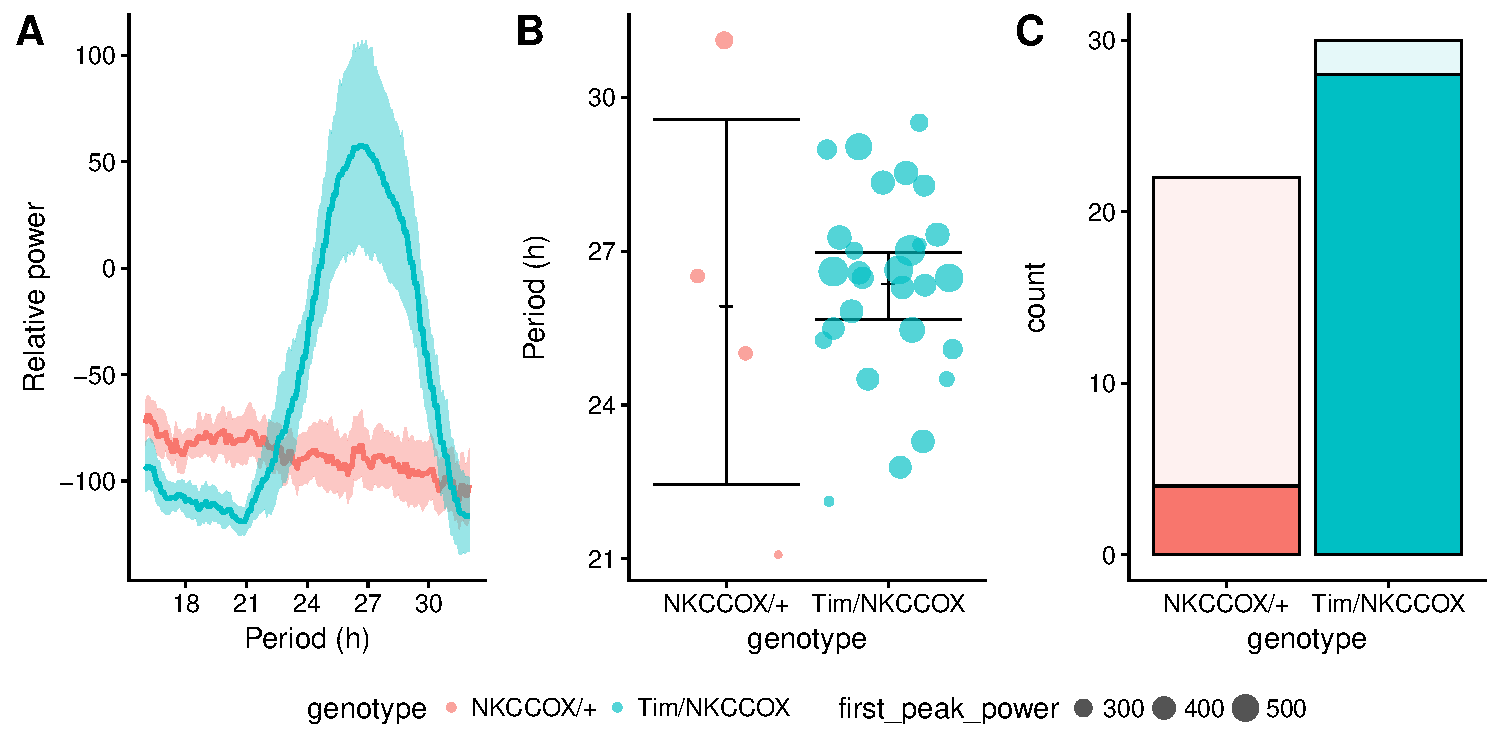
\includegraphics[width=1\textwidth]{fig/fig-4.pdf}
	\caption{{\bf Population statistics on circadian phenotype.}
			TODO}
	\label{fig:fig-4}
\end{figure}


* high scalability

* reproducibility

* from raw data to publication-quality figures

* flexibility




% We present an small example examining the circadian behaviour of 128 fruit flies in recorded in a DAM2 -- a paradigm very widely adopted. 
% A less formal description of this case and others are explained at \href{https://rethomics.github.io/}{https://rethomics.github.io/}.
% In order to prodive a more comprehensive and didactic example, data was altered and simplified.	
% Fig~\ref{fig:experiment} describes our case experiment (A) and the corresponding metadata (B).
% Briefly, three monitors were used each containing 16 males and 16 females of a different genotype (A, B and C).
% Two replicates were performed at different times.
% raw data and metadata files are publicly available TODO cite zenodo
% 

\section*{Availability and Future Directions}
All packages in the \texttt{rethomics} framework are available under the terms of the GPLv3 license and listed at
\href{https://github.com/rethomics}{https://github.com/rethomics/}.
Extensive installation instructions as well as reproducible demos and tutorials are available at
\href{https://rethomics.github.io/}{https://rethomics.github.io/}.
All packages are continuously integrated and unit tested on several version of \texttt{R} to minimise resent and future issues.

* Other inputs 

* Position analysis

* GUI

* ... 


\section*{Supporting information}

% Include only the SI item label in the paragraph heading. Use the \nameref{label} command to cite SI items in the text.
\paragraph*{S1 Fig.}
\label{S1-Fig}
{\bf Bold the title sentence.} Add descriptive text after the title of the item (optional).


\section*{Acknowledgements}
TODO:

Han Kim

Maite

Hannah 

Patrick Kr{\"a}tschmer


% Include only the SI item label in the paragraph heading. Use the \nameref{label} command to cite SI items in the text.
%\paragraph*{S1 Fig.}
%\label{S1_Fig}
%{\bf Bold the title sentence.} Add descriptive text after the title of the item (optional).

\nolinenumbers

% Either type in your references using
% \begin{thebibliography}{}
% \bibitem{}
% Text
% \end{thebibliography}
%
% or
%
% Compile your BiBTeX database using our plos2015.bst
% style file and paste the contents of your .bbl file
% here. See http://journals.plos.org/plosone/s/latex for 
% step-by-step instructions.
% 


\begin{thebibliography}{10}

\bibitem{bib1}
Conant GC, Wolfe KH.
\newblock {{T}urning a hobby into a job: how duplicated genes find new
  functions}.
\newblock Nat Rev Genet. 2008 Dec;9(12):938--950.

\bibitem{bib2}
Ohno S.
\newblock Evolution by gene duplication.
\newblock London: George Alien \& Unwin Ltd. Berlin, Heidelberg and New York:
  Springer-Verlag.; 1970.

\bibitem{bib3}
Magwire MM, Bayer F, Webster CL, Cao C, Jiggins FM.
\newblock {{S}uccessive increases in the resistance of {D}rosophila to viral
  infection through a transposon insertion followed by a {D}uplication}.
\newblock PLoS Genet. 2011 Oct;7(10):e1002337.

\end{thebibliography}



\end{document}

